\appendix \chapter{RadarPi Procedures}\label{chap:Tutorial}

\section{Set-Up}\label{Appendix:Tutorial}

The instructions followed in this section serves as a tutorial or a guide to assemble the Audio Radar in its entirety. It will follow initial setup of test equipment used, assembly of the transmitting and receiving hardware and finally the software component of the project will be addressed.

\subsection{Raspberry Pi Setup}

Complete setup instructions exist in many forms online however, this guide will serve the setup requirements needed only for the Audio Radar. Other functionality of the Raspberry Pi are ignored but it should be noted that it is not limited to only the functions that are used here. 

It is assumed that the following is available to the user:

\begin{itemize}
    \item Raspberry Pi 3 or newer\footnote{Models older than the Raspberry Pi 3 will also work but a USB WiFi dongle will be required.} with Raspbian with Desktop already installed and SSH enabled\footnote{Numerous online resources exist to achieve this such as \href{https://hackernoon.com/raspberry-pi-headless-install-462ccabd75d0}{\underline{this}.}}.
    \item A computer with keyboard, mouse, monitor and SD card slot
    \item An Ethernet cable
    \item A local area network with Ethernet communication and WiFi.
\end{itemize}

The setup of the Raspberry Pi is covered extensively on the internet. \href{https://www.instructables.com/id/Ultimate-Raspberry-Pi-Configuration-Guide/}{\textbf{Here}} is a guide to set up the Raspberry Pi.

\subsection{Package Installation and Setup}
The following packages need to be installed:

\begin{itemize}
\item Flask (\href{http://mattrichardson.com/Raspberry-Pi-Flask/}{\textbf{Link}})
\item PyGame (\href{https://www.pygame.org/wiki/GettingStarted}{\textbf{Link}})
\item $I^2S$ DAC Driver (\href{https://learn.adafruit.com/adafruit-max98357-i2s-class-d-mono-amp/overview}{\textbf{Link}})
\item RaspAP (\href{https://raspberry-valley.azurewebsites.net/RaspAP-Wifi-Hotspot/}{\textbf{Link}})
\item If the radar is implemented using something other than the Raspberry Pi, additional packages need to be installed: 
\begin{itemize}
\item Numpy (\href{https://scipy.org/install.html}{\textbf{Link}})
\item Scipy (\href{https://scipy.org/install.html}{\textbf{Link}})
\item Matplotlib (\href{https://scipy.org/install.html}{\textbf{Link}})
\end{itemize}
\end{itemize}

\subsection{Hardware Setup}
The following links would help with setting up all the hardware needed for the radar.
\begin{itemize}
\item Microphone setup (\href{https://learn.adafruit.com/adafruit-agc-electret-microphone-amplifier-max9814/wiring-and-test}{\textbf{Link}})
\item Speaker setup (\href{https://learn.adafruit.com/adafruit-max98357-i2s-class-d-mono-amp/overview}{\textbf{Link}})
\end{itemize}

\subsection{Procedure}
Clone repository that is linked in Appendix \ref{Appendix:Code} and copy contents to \verb /home/pi/Documents/ 
Set up script to run \verb webapp.py  at start up of Raspberry Pi (\href{https://www.instructables.com/id/Raspberry-Pi-Launch-Python-script-on-startup/}{\textbf{Link}}).

\newpage

\section{Usage Tutorial}
The radar was designed to be as simple as possible to use. Therefore, after initial set-up, the only instructions on how to use the radar are as follows:

\begin{enumerate}
\item Power the Raspberry Pi with a minimum $1.5\ A$ power supply.
\item Wait for 10 seconds until the Wi-Fi network 'RadarPi' is registered. 
\item Scan the QR-code with your device or connect to the Wi-Fi manually.
\item Scan the other QR-code to visit the web page or enter the web address manually.
\item Select a mode that you want to use i.e. Continuous Wave or Pulsed-Doppler. Both have a technical and non-technical option. The technical version is intended only for advanced users.
\item Enter the parameters requested by the web page.
\item Click 'submit' and wait for the resulting figure to appear. The Pulsed-Doppler has significant operations and may take longer than $8\ s$.
\item Click on the 'Home' button to return to the landing page or select another mode from the navigation bar.
\item When done using the RadarPi, simply disconnect the power cable from the Raspberry Pi.
\item If any issues arise, the GitHub page will remain active, where questions can be asked, as this project will continue with further developments after the conclusion of the course.
\end{enumerate}



\newpage

\chapter{Code}\label{Appendix:Code}

Code used for testing and creation of RadarPi: \url{https://github.com/DewanPieterse/AudioRadar}\\ \\
The GitHub page containing all code to set-up and run RadarPi: \url{https://github.com/DewanPieterse/RadarPi}\\ \\


\newpage

\chapter{Testing Procedures and Results}\label{chap:Testing}

\section{Testing Set-Up and Testing Results}
All of the recorded data sets to verify the testing of the microphones and speakers can be found along with all the screenshots and photos taken, \href{https://github.com/DewanPieterse/AudioRadar/tree/master/Matlab}{\underline{here}}. 

\begin{figure}[h!]
    \centering
    \begin{minipage}{0.45\textwidth}
        \centering
        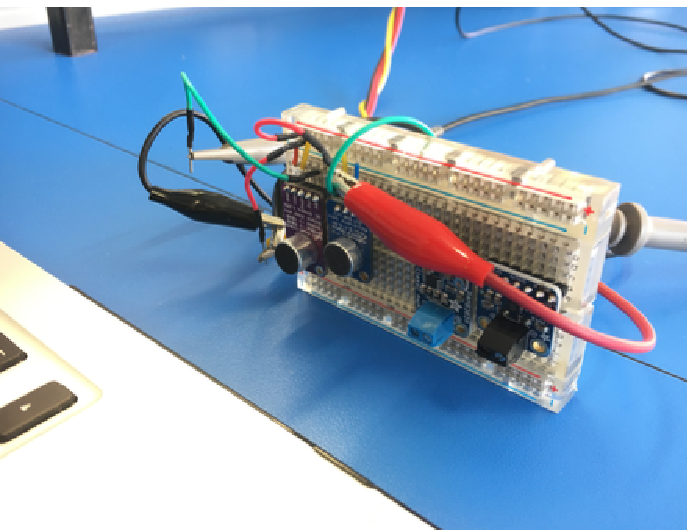
\includegraphics[width = 0.9\textwidth]{images/mic.pdf}
    \caption{Microphone Set-Up}\label{fig:mic}
    \end{minipage}\hfill
    \begin{minipage}{0.45\textwidth}
        \centering
        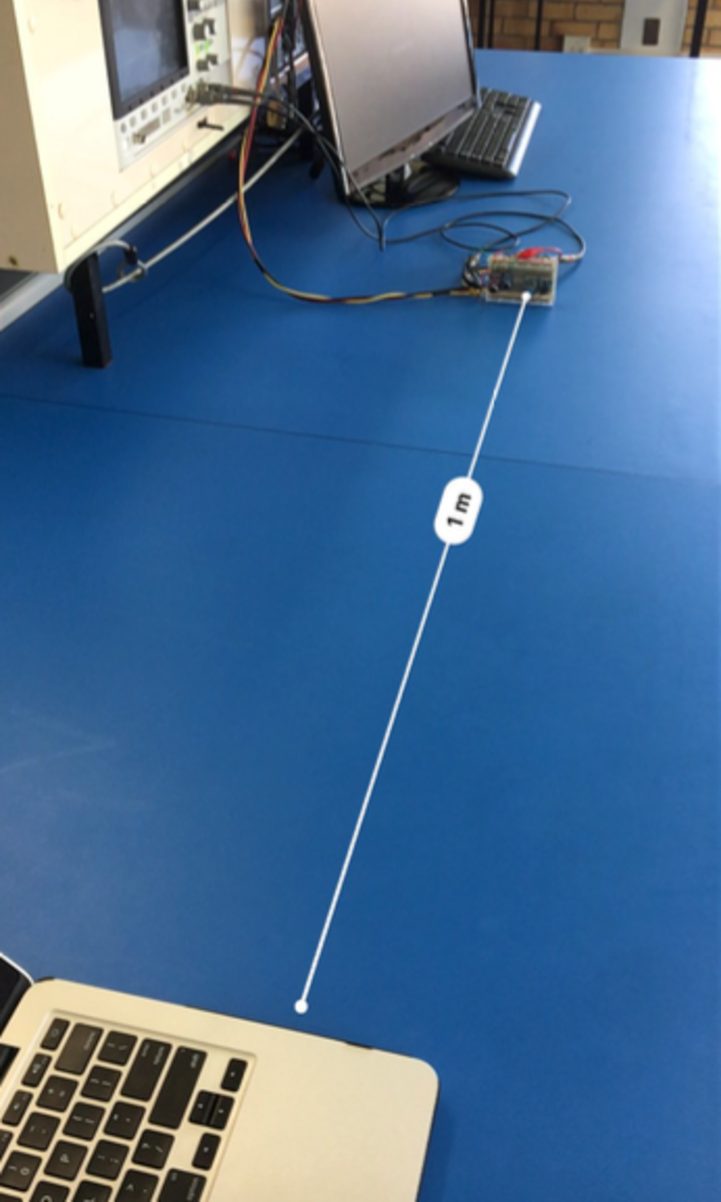
\includegraphics[width = 0.9\textwidth]{images/dist.pdf}
    \caption{Distance Measurement}\label{fig:measure}
    \end{minipage}
\end{figure}
\begin{figure}[h!]
    \centering
    \begin{minipage}{0.45\textwidth}
        \centering
       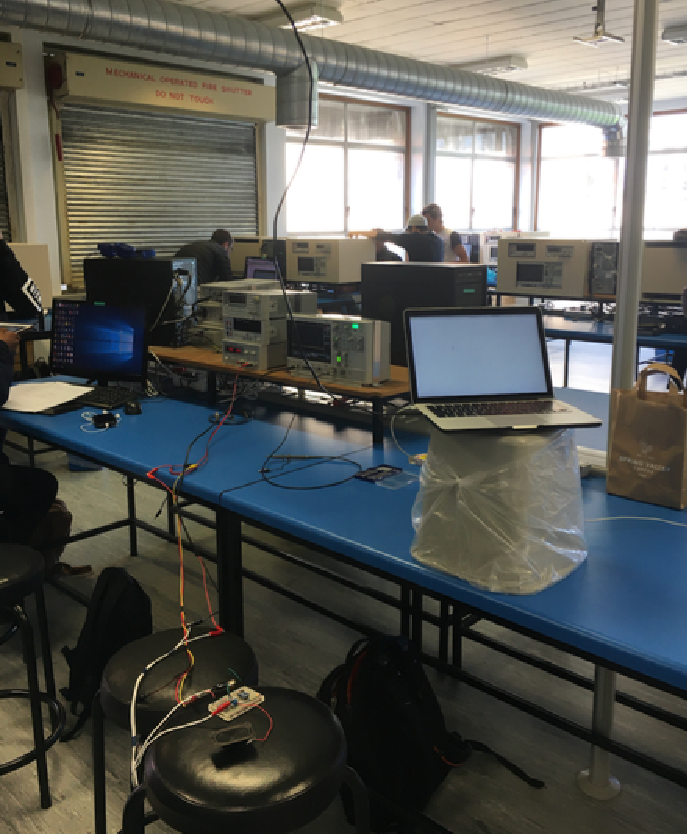
\includegraphics[width = 0.9\textwidth]{images/susp.pdf}
    \caption{Microphone Suspended}\label{fig:suspended}
    \end{minipage}\hfill
    \begin{minipage}{0.45\textwidth}
        \centering
        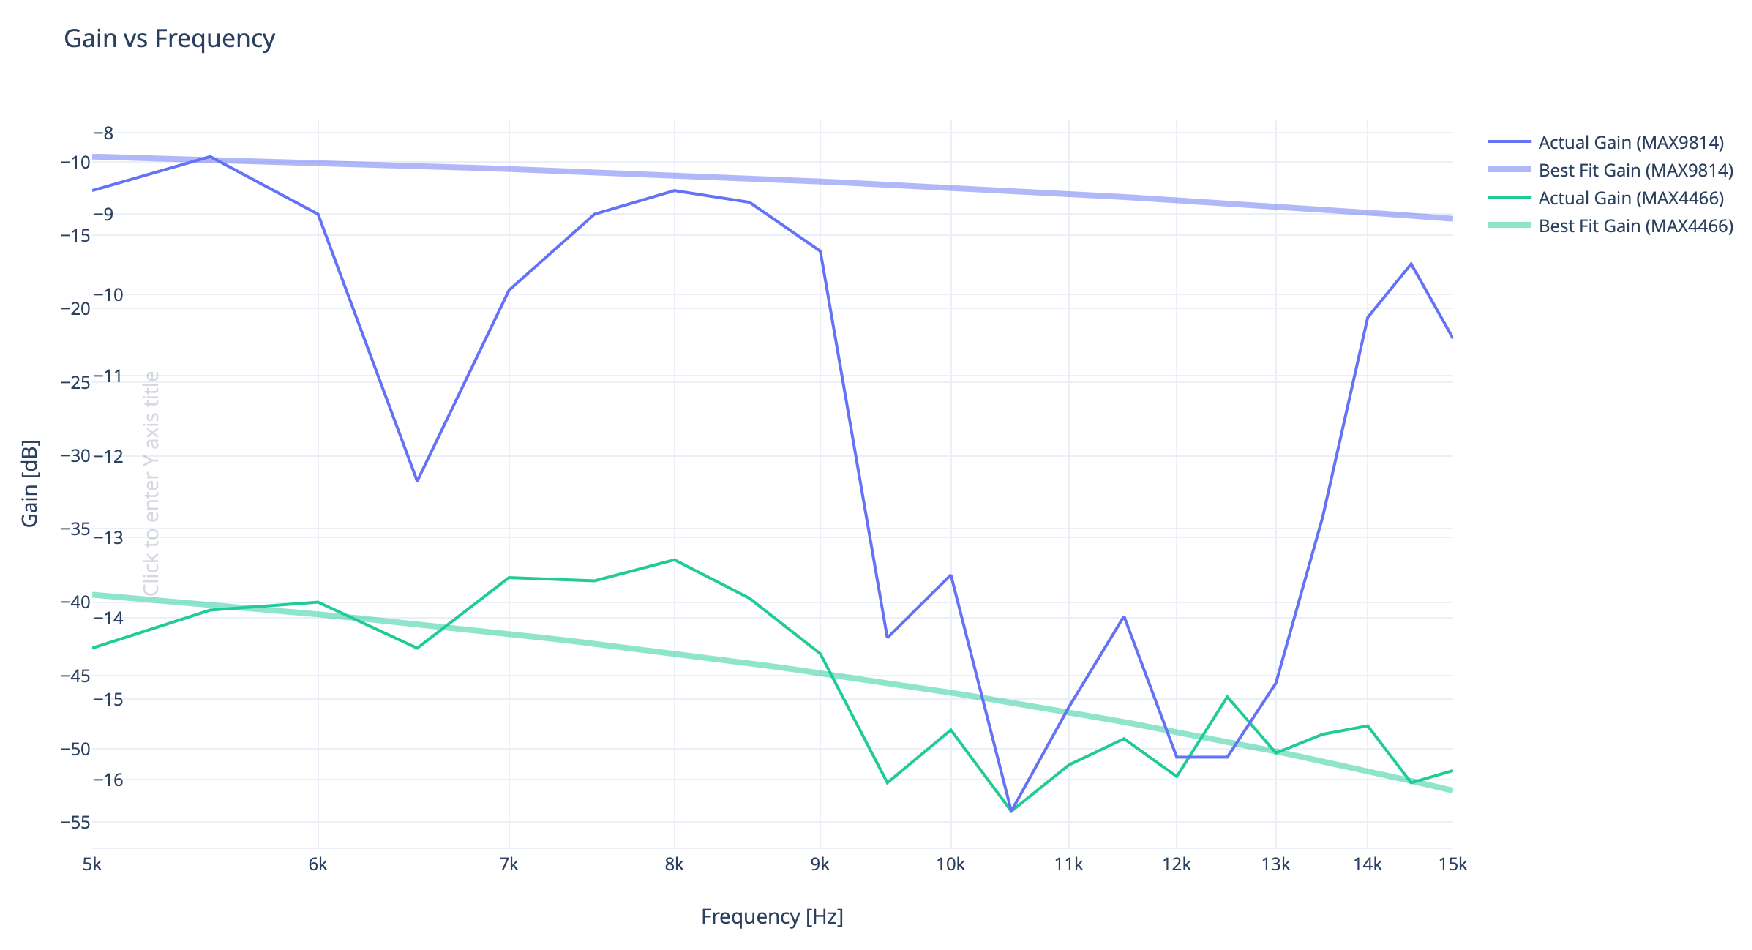
\includegraphics[width = 0.9\textwidth]{images/gainVSfreq.pdf}
    \caption{Initial gain vs frequencies: Microphones}\label{fig:gainVSfreq}
    \end{minipage}
\end{figure}

\begin{figure}[h!]
    \centering
    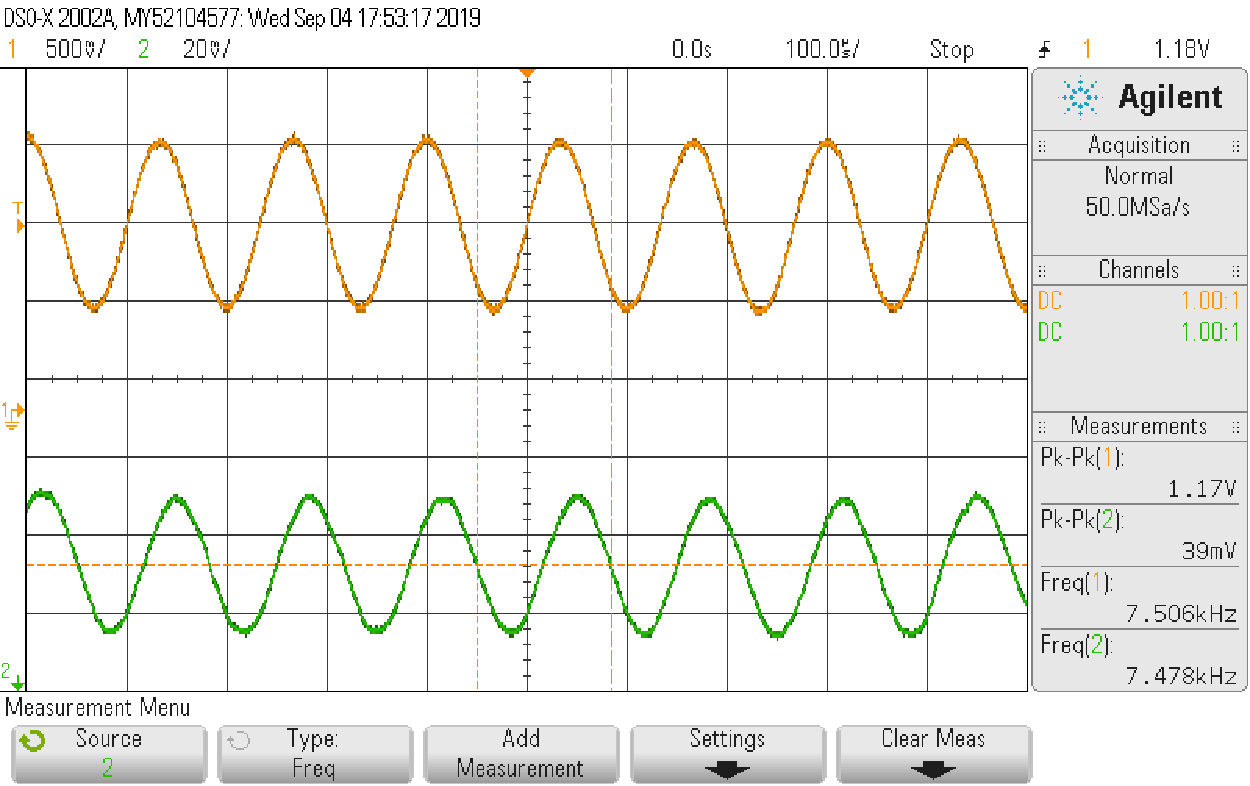
\includegraphics[width = 0.45\textwidth]{images/scope_5.pdf}
    \caption{Sample of Oscilloscope view when testing Speakers}\label{fig:scope_5}
\end{figure}
\newpage
\section{Experimentation Results\label{appendix:PDResults}}
Results from Pulse Doppler Radar mapping a room as from Section \ref{section:PDResults}

\begin{figure}[h!]
    \centering
    \begin{minipage}{0.45\textwidth}
        \centering
        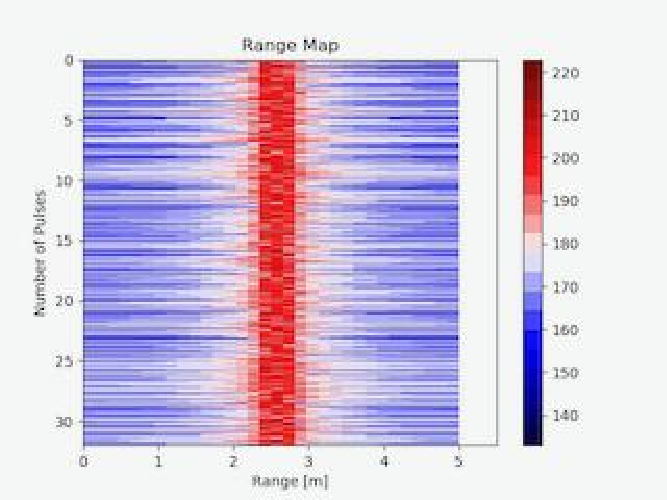
\includegraphics[width = 0.9\textwidth]{images/pulsedTest1-3.pdf}
        \caption{Measurement to Eastern wall in PD Test 1}\label{fig:PDResults3}
    \end{minipage}\hfill
    \begin{minipage}{0.45\textwidth}
        \centering
        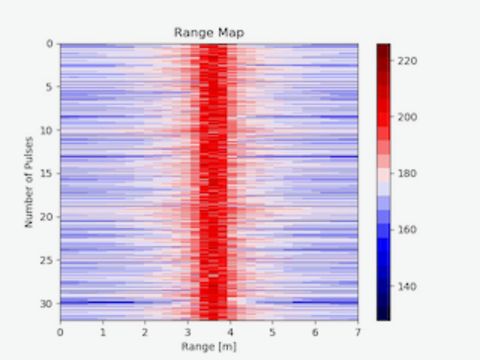
\includegraphics[width=0.9\textwidth]{images/pulsedTest1-4.pdf}
        \caption{Measurement to Southern wall in PD Test 1}\label{fig:PDResults4}
    \end{minipage}
\end{figure}

\newpage